\documentclass[a4paper,10pt]{article} % Default font size and paper size

%{{{ Packages & Includes
%\usepackage{xunicode,xltxtra,url,parskip} % Formatting packages
\usepackage{url,parskip} % Formatting packages
\usepackage{graphicx}
\usepackage{adjustbox}

\usepackage[usenames,dvipsnames]{xcolor} % Required for specifying custom colors

%\usepackage[big]{layaureo} % Margin formatting of the A4 page, an alternative to layaureo can be \usepackage{fullpage}
% To reduce the height of the top margin uncomment: \addtolength{\voffset}{-1.3cm}
\usepackage[left=2.5cm,right=2.5cm,top=2cm,bottom=2.5cm]{geometry}
\usepackage{hyperref} % Required for adding links	and customizing them
\definecolor{linkcolour}{rgb}{0,0.2,0.6} % Link color
\hypersetup{colorlinks,breaklinks,urlcolor=linkcolour,linkcolor=linkcolour} % Set link colors throughout the document
\usepackage{array}
\newcolumntype{R}[1]{>{\raggedleft\let\newline\\\arraybackslash\hspace{0pt}}m{#1}}
\newcolumntype{L}[1]{>{\raggedright\let\newline\\\arraybackslash\hspace{0pt}}m{#1}}
\newcolumntype{C}[1]{>{\centering\let\newline\\\arraybackslash\hspace{0pt}}m{#1}}

\usepackage{titlesec} % Used to customize the \section command
\titleformat{\section}{\scshape\raggedright}{}{0em}{}[\titlerule] % Text formatting of sections
\titlespacing{\section}{0pt}{3pt}{3pt} % Spacing around sections
%}}}

\begin{document}

\pagestyle{empty} % Removes page numbering

\section{Personal Information}

\begin{table}[ht]
\begin{minipage}{0.77\linewidth}
    \begin{tabular}{L{1.75cm}p{3cm}p{2cm}L{1.4cm}L{1.5cm}}
        Full Name: & \textbf{Carlos Segarra} & & \multicolumn{2}{l}{\textbf{Languages:}} \\
        Birthday: & 09/06/1996 & & Spanish: & Native\\
        Hometown: & Barcelona, Spain & & Catalan: & Native \\
        Residence: & Neuch\^atel, CH & & English: & C2\\
        Mail: & \small{carlossegarragonzalez@gmail.com} & & French: & Fluent \\
        Phone: & +41 79 935 05 41 & & German: & A2
    \end{tabular}
\end{minipage}\hfill
\begin{minipage}{0.2\linewidth}
\centering
%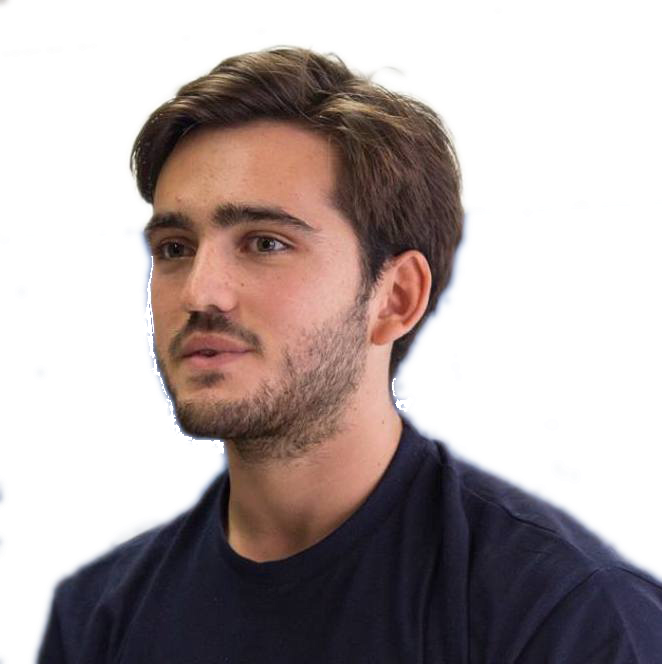
\includegraphics[width=2.5cm]{carlos_portrait.png}
{%
\setlength{\fboxsep}{0pt}%
\setlength{\fboxrule}{0.7pt}%
\fbox{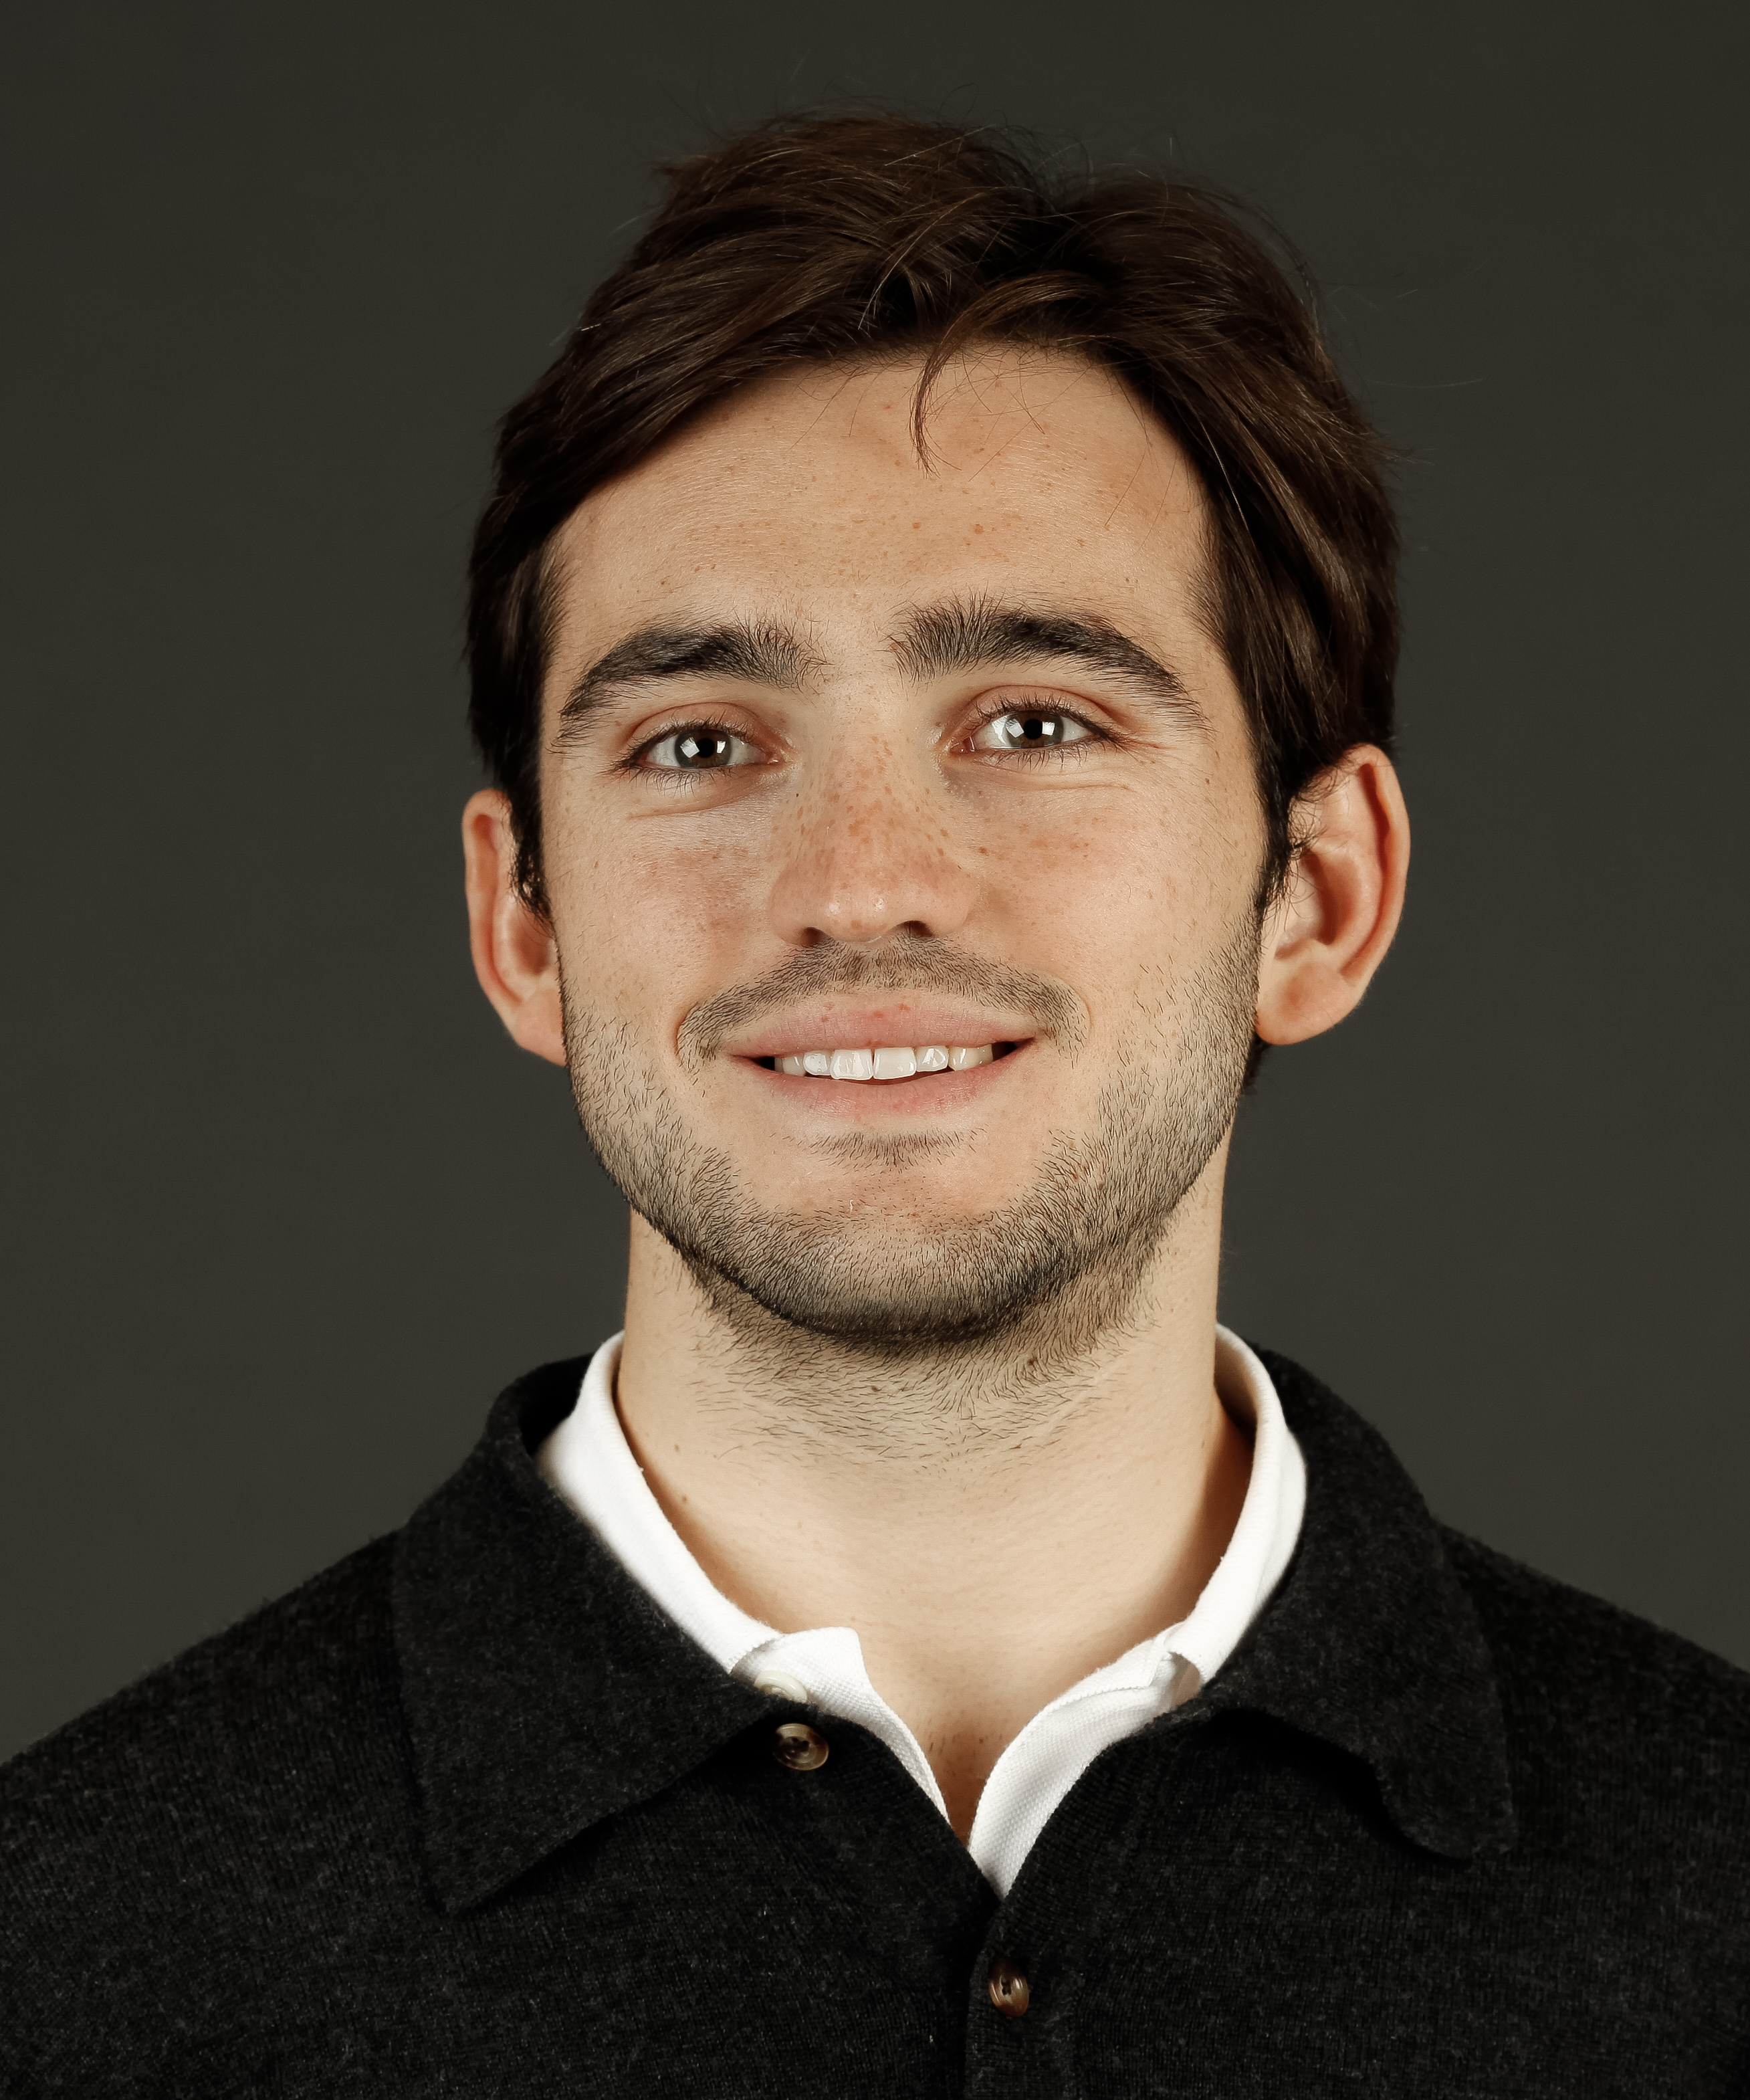
\includegraphics[width=2.5cm]{csem_img.jpg}}%
}%
\end{minipage} 
\end{table}

\section{Publications}
\begin{tabular}{p{15.2cm}}
    C. Segarra, M. Lemay, R. Delgado-Gonzalo, and V. Schiavoni, \textbf{\textit{"\textsc{MedSpark}: Using Trusted Execution Environments for Secure Stream Processing of Medical Data"}}. DAIS'19, Copenhagen, Denmark, June 17-21, 2019. \\[3pt]
    C. Segarra, E. Muntan\'e, M. Lemay, V. Schiavoni, and  R. Delgado-Gonzalo, \textbf{\textit{"\textsc{MedSpark}: Secure Stream Processing for Medical Data"}}. IEEE EMBC'19, Berlin, Germany, July 23-27, 2019. \\
\end{tabular}

\section{Work Experience}
%
\begin{tabular}{R{1.5cm}|p{13.8cm}}
    \emph{Current} & Trainee at the \textbf{\textsc{Swiss Center for Electronics and Microtechnology} (CSEM)} \\
    \textsc{10/2018} & \small{\emph{Embedded Software Division} - Sup. Ricard Delgado Gonzalo, PhD }\\ 
& \footnotesize{Intern at the Embedded Software Division of the CSEM in Neuch\^atel, CH, using Trusted Execution Environments to perform privacy-preserving computations on IoT medical devices. Developed a distributed streaming platform on Intel SGX and now working on leveraging Arm TrustZone to implement a secure version of the MQTT protocol.}
\end{tabular}

\begin{tabular}{R{1.5cm}|p{13.8cm}}
    \textsc{09/2018} & Trainee at \textbf{\textsc{Nokia Bell Labs}} \\
    \textsc{06/2018} & \small{\emph{Security Group} - Sup. Matteo Signorini, PhD and Matteo Pontecorvi, PhD}\\ 
& \footnotesize{Summer intern at the the Cybersecurity department at Nokia Bell Labs in Paris-Saclay, France. I developed a graph-based model to detect, cluster and classify chains of malicious transactions in the Bitcoin's Blockchain. By defining an abstraction layer atop the chain and an isomorphism class, we managed to identify a variety of services.}
\end{tabular}

\begin{tabular}{R{1.5cm}|p{13.8cm}}
    \textsc{06/2018} & Research Student at the \textbf{\textsc{Barcelona Supercomputing Center} (BSC)} \\
    \textsc{04/2017} & \small{\emph{Workflows and Distributed Computing Group} - Sup. Rosa M. Badia, PhD} \\ 
    & \footnotesize{Research student at the Workflows and Distributed Computing Group at the BSC in Barcelona, Spain. I developed, deployed and benchmarked a distributed implementation of the DBSCAN algorithm using COMP Superscalar, a programming model for distributed computing. Evaluation was done in the \textit{Mare Nostrum} supercomputer.}
\end{tabular}

\section{Education}

\begin{tabular}{R{1.5cm}|p{13.8cm}}	
    \textsc{05/2019} & Bachelor's degree in \textbf{\textsc{Mathematics}} \\ 
    \textsc{09/2014} & \small{\emph{Polytechnic University of Catalonia}, UPC}\\
     & \footnotesize{BSc in Mathematics within a double degree program in the Interdisciplinary Higher Education Center (CFIS) at the UPC. Relevant coursework covers real and complex analysis, statistics, probability and graph theory, combinatorics and algorithms.}
\end{tabular}

\begin{tabular}{R{1.5cm}|p{13.8cm}}	
    \textsc{05/2019} &  Bachelor`s degree in \textbf{\textsc{Telecommunications Science and Technology}}\\ 
    \textsc{09/2014} & \small{\emph{Polytechnic University of Catalonia}, UPC} \\
     & \footnotesize{BSc in Telecommunications Engineering within a double degree program in the Interdisciplinary Higher Education Center (CFIS) at the UPC. Relevant coursework covers networking and concurrency, digital and analogical communications and real time digital signal processing.}
\end{tabular}

%\begin{tabular}{R{1.5cm}|p{13.8cm}}	
%    \textsc{05/2014} & Spanish Baccalaureate \\
%    \textsc{09/2013} & \small{\emph{Escola Betània-Patmos}, Barcelona} \\ 
%    &  Graduated with honors. \\
%\end{tabular}

\section{Skills and Interests}

\begin{tabular}{R{1.5cm}|p{13.8cm}}
      %& \textbf{Distributed Systems} \\ %\textsc{DS}
    & {My main background and interests comprise \textbf{distributed} and \textbf{decentralized} systems. I am also particularly interested in \textbf{cryptography}, \textbf{security} and \textbf{data privacy}, specially in homomorphic encryption and trusted execution environments. Furthermore, \textbf{graph theory}, \textbf{combinatorics} and \textbf{probability} are math disciplines that I enjoy. In short, I am very interested in applying strong and founded mathematical concepts to distributed computing environments. On a lighter note, I read literature of all sorts and I train for and take part in amateur triathlons.}  \\
\end{tabular}

%\begin{tabular}{R{1.5cm}|p{13.8cm}}
%      & \textbf{Security and Data Privacy} \\ %\textsc{BD}
%    & \footnotesize{The constant exposure we have to computers and the amount of data these process, makes ensuring security and privacy of vital importance. I am particularly interested in Trusted Execution Environments and Homomorphic Encryption for privacy-preserving computing techniques, and everything concerning data-at-rest and in-motion's security.}  \\
%\end{tabular}
%
%\begin{tabular}{R{1.5cm}|p{13.8cm}}
%      & \textbf{Graph Theory and Combinatorics} \\ %\textsc{GT \& C}
%    & \footnotesize{I am strongly interested in the areas of mathematics studying graphs, combinatorics and probability. I specially like the impact of these in distributed systems, coding theory and cryptography.}  \\
%\end{tabular}
%
%\begin{tabular}{R{1.5cm}|p{13.8cm}}
%      & \textbf{Other Interests} \\ %\textsc{OI}
%    & \footnotesize{On a lighter note, I also enjoy reading literature of all sorts. It allows me to maintain a global perspective whilst working on very particular topics. I train for and take part in amateur triathlons.}  \\
%\end{tabular}
\end{document}
